% begin module differential-def
\begin{frame}
\frametitle{Differentials}
\begin{itemize}
\item  Sometimes the ideas of linear approximation are expressed using differentials.
\item  Let $y = f(x)$, where $f$ is differentiable.
\item  You are already familiar with the variable $\Delta y$ (the ``rise''), which depends on $x$ and $\Delta x$ (the ``run''), according to
\[
\Delta y = f(x + \Delta x) - f(x)
\]
\item  In differential notation, we name the ``run'' $\diff x = \Delta x$.  This is an independent variable, much like $x$ itself.
\item  $\diff y$ is a dependent variable that depends on $x$ and $\diff x$.
\item  It measures the ``rise'' for the linear approximation $L(x)$:
\end{itemize}
\begin{align*}
\uncover<1->{%
\diff y%
}%
& \uncover<1->{ = } %
\uncover<1->{%
L(x+\diff x) - L(x)%
}%
%\\%
%& \uncover<2->{ = } &%
%\uncover<2->{%
%[f(x) + f'(x)(x+\diff x - x)] - [f(x) + f'(x)(x-x)]%
%}\\%
%& \uncover<2->{ = } &%
%\uncover<2->{%
%f'(x)\diff x%
%}\\%
\end{align*}
\end{frame}


\begin{frame}
\begin{center}%
\ \only<handout:1| -2>{%
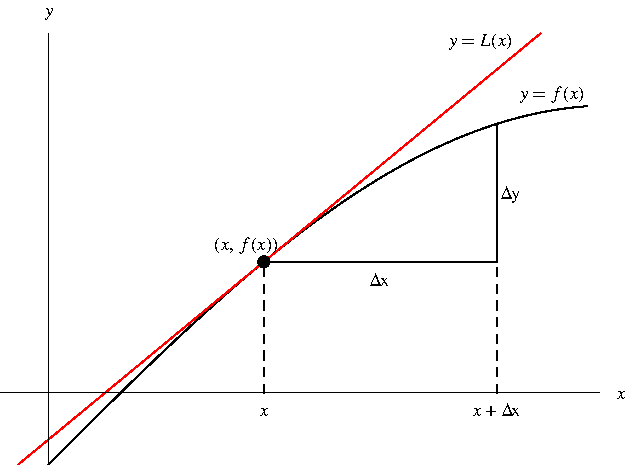
\includegraphics[width=7cm]{differentials/pictures/03-09-differentiala.pdf}%
}%
\only<handout:2| 3->{%
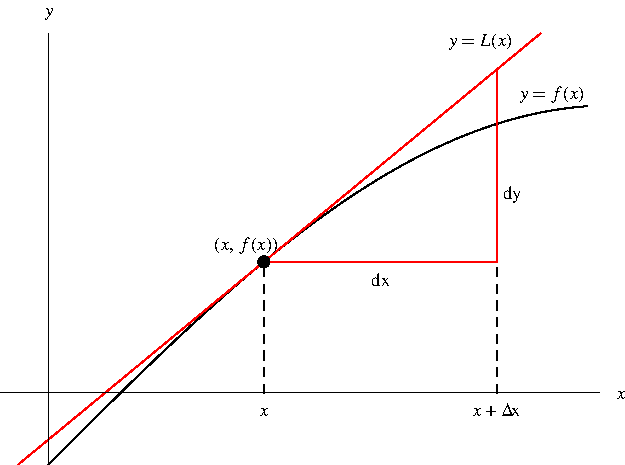
\includegraphics[width=7cm]{differentials/pictures/03-09-differentialb.pdf}%
}%

\begin{tabular}{|l|c|c|}
\hline
Function & \alert<handout:1| 2>{$f$} & \alert<handout:2| 3>{$L$}\\
\hline
Run & \alert<handout:1| 2>{$\Delta x$} & \alert<handout:2| 3>{$\diff x$}\\
Rise & \alert<handout:1| 2>{$\Delta y$} & \alert<handout:2| 3>{$\diff y$}\\
Formula & \alert<handout:1| 2>{$\Delta y = f(x+\Delta x) - f(x)$} & \alert<handout:2| 3>{$\diff y = L(x+\diff x) - L(x)$}\\
\hline
\end{tabular}
\end{center}%

\uncover<4->{%
Easier formula: $\diff y = f'(x)\diff x$.
}%
\end{frame}
% end module differential-def
